\section{Ausführung Online Umfrage}
\label{sec:ausfuehrung-online-umfrage}
Im Folgenden werden die Fragen und Antworten der Online Umfrage ausführlich dargestellt. Die Durchführung und Ergebnisse sind in Kapitel \ref{subsec:online-umfrage} zusammengefasst.

\begin{enumerate}
    \item \textbf{Verwenden Sie Online Banking?} \\ Anzahl Teilnehmer: 48
    \begin{itemize}
        \item[] 44 (91.7\%): ja
        \item[] 4 (8.3\%): nein
    \end{itemize}
    
    \item \textbf{Was müsste sich ändern, damit Sie es verwenden würden?}\\ Anzahl Teilnehmer: 3
    \begin{itemize}
        \item[] Nichts
        \item[] Sicherheitsproblematik
        \item[] Wenn mir jemand beim Einrichten hilft, würde ich es sofort verwenden
    \end{itemize}
    
    \item \textbf{Was sind Ihre Hauptgründe für die Nutzung von Online Banking?}\\ Anzahl Teilnehmer: 44
    \begin{itemize}
        \item[] 16 (36.4\%): Öffnungszeiten der Banken
        \item[] 36 (81.8\%): Schnell
        \item[] 10 (22.7\%): Kostengünstig
        \item[] 23 (52.3\%): Überall Zugriff
        \item[] 34 (77.3\%): Bequem
        \item[] 0 (0.0\%): Andere
    \end{itemize}
    
     \item \textbf{Aus welchen konkreten Gründen prüfen Sie Ihren Kontostand bzw. Ihre Umsatzanzeige?}\\ Anzahl Teilnehmer: 44
     \begin{itemize}
        \item Abbuchungen
        \item Aktuelles Guthaben
        \item Kontrolle
        \item Aktualität: Was ist drauf was wird abgebucht was kann ich mir noch leisten
        \item Kontrolle
        \item Um auf dem aktuellen Stand zu sein
        \item Um zu prüfen
        \item Zur Überwachung
        \item Um zu sehen ob alles richtig läuft
        \item Damit man die Kosten immer im Auge hat
        \item Übersicht
        \item Kontostand
        \item Allgemeiner Überblick vor Überweisungen
        \item Um immer zu wissen wie viel Geld man hat und um den Cashflow im Auge zu haben
        \item Kontrolle
        \item Damit ich weiß, wieviel Geld noch auf dem Konto ist bzw. ob Auffälligkeiten sind
        \item Ob alle Daueraufträge korrekt sind und nichts falsch abgebucht wird
        \item Fehlbuchungen Kontrolle über Ausgaben
        \item damit nicht unbefugtes abgebucht wird
        \item ob Lohn da ist
        \item ob ich evtl. Geld aus Gutschriften etc. erhalten hab
        \item Um auf dem Laufenden über meinen Kontostatus zu haben
        \item Zahlungs ein-/ausgabekontrolle von onlineshopping
        \item Papier sparen
        \item Vermeidung von Missbrauch und einfache Übersicht
        \item Kontrolle zu Ein und Ausgaben
        \item Übersicht Barvermögen, Lastschriften überwachen
        \item Um den Kontostand zu erfahren und über den Zahlungsverkehr auf dem Laufenden zu sein
        \item Sicherheit
        \item Den aktuelle Kontostand im Blick haben
        \item Um zu sehen wie viel Geld auf dem Konto ist
        \item Um Überblick auf alle Transaktionen zu haben
        \item Um nicht ins Minus zu rutschen
        \item Sind die Abbuchungen erlaubt
        \item Sind Einnahmen überwiesen
        \item Um falsche Abbuchungen zu vermeiden Den Kontostand im Blick zu haben
        \item Prüfung von Fehlbuchungen
    \end{itemize}
    
     \item \textbf{Führen Sie mit Online Banking Überweisungen durch?} \\ Anzahl Teilnehmer: 44
    \begin{itemize}
        \item[] 44 (100\%): ja
        \item[] 0 (0\%): nein
    \end{itemize}
    
     \item \textbf{In welcher Form führen Sie Überweisungen durch? (mehrere Antworten möglich)} \\ Anzahl Teilnehmer: 44
    \begin{itemize}
        \item[] 22 (50.0\%): Unter Verwendung von Überweisungsvorlagen
        \item[] 37 (84.1\%): Überweisungsformular ausfüllen
        \item[] 27 (61.4\%): Daueraufträge einrichten
    \end{itemize}
    
     \item \textbf{Welches TAN Verfahren verwenden Sie dabei?} \\ Anzahl Teilnehmer: 44
    \begin{itemize}
        \item[] 1 (2.3\%): iTAN (Liste)
        \item[] 20 (45.5\%): mTAN (SMS)
        \item[] 17 (38.6\%): smartTAN (EC Kartenleser)
        \item[] 4 (9.1\%): pushTAN (Smartphone App)
        \item[] 2 (4.5\%): Andere 
        \item[] Antworten aus dem Zusatzfeld: 
        \begin{itemize}
            \item[] Chip Tan
            \item[] Sowohl mtan und pushTAN
        \end{itemize}
    \end{itemize}
    
    \item \textbf{Nutzen Sie ein Finanzmanagement- System, um Ihre Kontodaten über längere Zeiträume auszuwerten?} \\ Anzahl Teilnehmer: 44
    \begin{itemize}
        \item[] 9 (20.5\%): ja
        \item[] 35 (79.5\%): nein
    \end{itemize}
    
    \item \textbf{Welche Funktionen verwenden Sie dabei? (mehrere Antworten möglich)} \\ Anzahl Teilnehmer: 9
    \begin{itemize}
        \item[] 2 (22.2\%): Anlegen und Verwalten von Sparzielen/Budgets
        \item[] 8 (88.9\%): Auswertung Ihrer Umsätze
        \item[] 0 (0.0\%): Andere
    \end{itemize}
    
     \item \textbf{Investieren Sie in Aktien?} \\ Anzahl Teilnehmer: 44
    \begin{itemize}
        \item[] 9 (20.5\%): ja
        \item[] 35 (79.5\%): nein
    \end{itemize}
    
    \item \textbf{Verwenden Sie ein Online Portal für die Verwaltung Ihrer Aktien?} \\ Anzahl Teilnehmer: 10
    \begin{itemize}
        \item[] 4 (40.0\%): ja
        \item[] 6 (60.0\%): nein
    \end{itemize}
    
     \item \textbf{Nach welchen Kriterien wählen Sie neue AKtien aus?}\\ Anzahl Teilnehmer: 8
     \begin{itemize}
        \item nach der Rendite unter Berücksichtigung des Risikos
        \item o.A.
        \item Risiko
        \item Aktien, die neu auf den Markt kommen
        \item Aktien die hohe Dividende bieten
        \item Aktien von weltbekannten Firmen wie z.B. Siemens, Coca Cola, etc.
        \item Kgv
        \item Nach Analyse von mir selbst
        \item Broker Informationen
        \item Blue Chips
        \item Branchenmix
    \end{itemize}
    
    \item \textbf{Welche Informationen Ihrer Aktien rufen Sie regelmäßig ab?}\\ Anzahl Teilnehmer: 8
     \begin{itemize}
        \item Kosten und Gewinn
        \item o.A.
        \item Sicherheit und Transparenz
        \item aktuelle Kurse
        \item Höchst und Niedrigkurs der letzten 12 Monate
        \item Kurs Chart der letzten fünf Jahre
        \item Kurs
        \item News der investierten Aktien
        \item Aktueller Stand
        \item Kurs
        \item Wirtschaftspresse
        \item Online Informationen
    \end{itemize}
    
     \item \textbf{Haben Sie bei der Nutzung von Online Banking sicherheitsrelevante Bedenken? Wenn ja welche? (mehrere Antworten möglich)} \\ Anzahl Teilnehmer: 43
    \begin{itemize}
        \item[] 22 (51.2\%): Account Sicherheit
        \item[] 2 (4.7\%): Cookies
        \item[] 30 (69.8\%): Hacker
        \item[] 11 (25.6\%): Identitätsraub
        \item[] 6 (14.0\%): Internet Verbindung
        \item[] 10 (23.3\%): Keine Bedenken
        \item[] 0 (0.0\%): Andere 
    \end{itemize}
    
     \item \textbf{Wie könnte Online Banking für Sie effizienter ablaufen?}\\ Anzahl Teilnehmer: 43
     \begin{itemize}
        \item Kartenleser schlecht abzulesen
        \item Keine Ahnung
        \item Für solche Fragen gibt es Leute wie dich hehe
        \item Es ist effizient genug
        \item Gar nicht. Hacker Probleme wird es immer geben...
        \item noch effizienter?
        \item Prinzipiell läuft es gut, nur werden Anwendungen schon angeboten, die teilweise noch nicht ganz ausgereift sind (z.B. Rechnungsscan)
        \item Keine Ahnung
        \item ?
        \item Ist i.O.!
        \item Mehrere Unterkonten in einem Konto, um das Geld für verschiedene Themen aufzuteilen (z.B. Lebensmittel, Versicherungen, sparen usw.)
        \item Keine Ahnung
        \item Bin bisher zufrieden
        \item Keine Ideen und Vorschläge
        \item Für mich ist es schon effizient
        \item Durch Fingerabdruck/Augenscan anstatt Password beim Login
        \item Sicherheit und gleichzeitig Handling verbessern
        \item ist effizient genug
        \item Deutliche Qualitäts- und Sicherheitssteigerung in Apps
        \item Schnellere aktualisierung der Kontostände
        \item eventuell Benachrichtigung bei ankommenden/abgehenden Geld per app
        \item USB Kartenleser um das umständliche halten des EC Kartenlesers zu vermeiden
        \item Schnellere Auswertung vom TAN Generator
        \item Weiß nicht
        \item aktuelle keine Verbesserung am Onlinebanking - Verfahren notwendig
        \item Aktuell bin ich zufrieden
        \item Zugriffe auch für alle Sparbücher, Konten usw.
        \item Könnte schneller sein die Formulare auszufüllen
        \item Überweisungen über Handy app mit digitale überweisungsformular so dass man nur noch bestätigen muss. Gleichzeitig MUSS das System 1000\% sicher sein.
        \item Depotdaten sollten besser ausgewertet sein
        \item Stärkere Verzahnung des Online-Auftritts mit dem persönlichen Kontakt in der Filiale (\zB Terminvereinbarungen, ToDos aus den Termin tracken etc.)
    \end{itemize}
    
    \item \textbf{Wie alt sind Sie?} \\ Anzahl Teilnehmer: 43
    \begin{itemize}
        \item[] 0 (0.0\%): unter 18 Jahre
        \item[] 20 (46.5\%): 18 - 30 Jahre
        \item[] 12 (27.9\%): 31 - 40 Jahre
        \item[] 6 (14.0\%): 41 - 50 Jahre
        \item[] 4 (9.3\%): 51 - 60 Jahre
        \item[] 1 (2.3\%): über 60 Jahre
    \end{itemize}
\end{enumerate}

\section{Interview Einverständniserklärung}
\label{sec:ausfuehrung-interview-einverstaendnis}
Die folgende Einverständniserklärung wird den Teilnehmern vor der Durchführung des Interviews zur Unterschrift vorgelegt. Die Durchführung der Interviews ist in Kapitel \ref{subsec:interviews} genauer beschrieben. \\

\textbf{Einverständniserklärung zum Interview}\\

Forschungsprojekt: Sprachassistenzsysteme im Bankkontenmanagement\\
Durchführende Institution: \adorsys \\
Projektleitung: Steffen Blümm\\
Interviewerin/Interviewer: Julian Wölk\\
Interviewdatum:\\\\
Ich erkläre mich dazu bereit, im Rahmen des genannten Forschungsprojekts an einem Interview teilzunehmen. Ich wurde über das Ziel und den Verlauf des Forschungsprojekts informiert. Ich kann das Interview jederzeit abbrechen, weitere Interviews ablehnen und meine Einwilligung in eine Aufzeichnung und Niederschrift des/der Interviews zurückziehen, ohne dass mir dadurch irgendwelche Nachteile entstehen.\\
Ich bin damit einverstanden, dass das Interview mit einem Aufnahmegerät aufgezeichnet und sodann von den Mitarbeiterinnen und Mitarbeitern des Studienprojekts in Schriftform gebracht wird. Für die weitere wissenschaftliche Auswertung des Interviewtextes werden alle Angaben zu meiner Person aus dem Text entfernt und/oder anonymisiert. Mir wird außerdem versichert, dass das Interview in wissenschaftlichen Veröffentlichungen nur in Ausschnitten zitiert wird, um sicherzustellen, dass ich auch durch die in den Interviews erzählte Reihenfolge von Ereignissen nicht für Dritte erkennbar werde.

\vspace{3cm}

Ort, Datum, Unterschrift


\section{Interview Fragebogen}
\label{sec:ausfuehrung-interview-fragebogen}
Folgende Fragen werden den Interview Teilnehmern gestellt. Weitere Informationen zur Durchführung sind in Kapitel \ref{subsec:interviews}.

\begin{enumerate}
    \item Wie alt sind Sie?
    \item Wie ist Ihre Haltung zu Sprachassistenten?
    \item Hatten Sie bereits mit Sprachassistenten zu tun?
    \begin{enumerate}
        \item Wofür haben Sie diese verwendet?
        \item Was finden Sie positiv an Sprachassistenten?
        \item Was hat Ihnen bei der Nutzung nicht gefallen?
    \end{enumerate}
    \item Wie greifen Sie auf Ihr Bankkonto hauptsächlich zu?
    \item Wenn Sie Ihren Kontostand bzw. Ihre Umsatzanzeige prüfen, welche Intention haben Sie dabei?
    \item Wenn Sie Sprachassistenten in Verbindung mit Online Bankkonten Management hören, was kommt Ihnen dabei in den Sinn?
    \item Wie sieht Ihr Umfeld aus, wenn Sie auf Ihr Bankkonto zugreifen?
    \item Suche nach Formulierungen
    \begin{enumerate}
        \item Was würden Sie ein Bankkonto fragen?
        \item Wie würden sie nach dem Folgenden Fragen:
        \begin{enumerate}
            \item Kontostand
            \item Verdeckter Ausgabe des Kontostandes
            \item Gehaltseingang
            \item Spezielle Umsätzen
            \item Budget/Fixkosten
            \item Sparziel anlegen
            \item An Sparziel überweisen
            \item Sparziel Status
        \end{enumerate}
        \item Fällt Ihnen sonst noch etwas ein?
    \end{enumerate}
    \item Wie ist Ihre Meinung zu so einem System?
    \item Würden Sie ein solches System verwenden?
    \item Welche Bedenken hätten Sie?
    \item Fällt Ihnen sonst noch etwas zu dem Thema ein?
\end{enumerate}

\section{Interview Auswertung}
\label{sec:ausfuehrung-interview-auswertung}
Die schriftliche Auswertung der Interviews ist stichpunktartig und sinngemäß unter Verwendung eigener Worte dokumentiert. Damit, wie in der Einverständniserklärung aus \ref{sec:ausfuehrung-interview-einverstaendnis} vereinbart, keine Rückschlüsse auf die Teilnehmer gezogen werden können, ist zudem die Anordnung der Antworten zufällig gewählt und entspricht keinem chronologischen Muster. 

\begin{enumerate}
    \item Altersgruppe 22 - 26
    \item Meinungen zu Sprachassistenten
    \begin{itemize}
        \item Eher skeptisch
        \item Cool wenn es funktioniert
        \item Missbrauch von Daten hat man nicht im Griff
        \item Grundsätzlich gut und praktisch, wenn es anständig funktioniert
        \item Erspart Tipparbeit
        \item Befremdlich
        \item Erleichtert vieles
        \item Es ist cool, mit Maschinen zu sprechen
    \end{itemize}
    \item Nur ein Teilnehmer hat Sprachassistenten bereits genutzt (Suchanfragen über Smartphone)
    \item Zugriff auf Bankkonto
    \begin{itemize}
        \item Erfolgt bei allen Teilnehmern über Online Banking am Rechner
        \item In Ausnahmesituationen auch über Smartphone (zum Beispiel Urlaub)
        \item Weg zur Bank nur bei Einzahlungen
    \end{itemize}
    \item Intentionen beim Prüfen von Kontostand und Umsatzdaten
    \begin{itemize}
        \item Überprüfen/Überwachen
        \item Ein- und Ausgang von Transaktionen prüfen
        \item Telefon Rechnung Mitte des Monats prüfen
        \item Gehaltseingang prüfen
        \item Kontoübersicht
        \item Prüfen des Guthabens vor dem Kauf bestimmter Dinge
        \item Stand am Monatsende prüfen
        \item Umssatzdaten speichern
    \end{itemize}
    \item Meinungen zu Sprachassistent in Verbindung mit Bankkonten Management
    \begin{itemize}
        \item Überwiegend Sicherheitsbedenken
        \item Angst vor Stimmen Fälschung, Missbrauch
        \item Vereinfachte Umsatzabfragen
        \item Schneller Zugriff auf Informationen
        \item Erspart Tipp- und Klickarbeit
        \item Praktisch
        \item Vorsicht bei Nutzung neuer Technologien
    \end{itemize}
    \item Teilnehmer sind während Ihrer Online Banking Tätigkeiten überwiegend alleine
    \item Szenarien für das Finden von Formulierungen
    \begin{enumerate}
        \item Kontostand
        \begin{itemize}
            \item Kontostand verdeckt ausgeben
            \item Wie ist mein Kontostand?
            \item Wie schaut mein aktueller Kontostand aus?
        \end{itemize}
        \item Gehaltseingang
        \begin{itemize}
            \item Ist das Gehalt eingegangen
            \item Zeig mir die eingegangenen Gehälter von Firma X
        \end{itemize}
        \item Spezielle Umsätzen
        \begin{itemize}
            \item Hat Kontoinhaber/Firma X schon abgebucht?
            \item Was sind die ein und ausgegangenen Buchungen?
            \item Wurde schon die Überweisung von gestern abgebucht?
        \end{itemize}
        \item Budget/Fixkosten
        \begin{itemize}
            \item Wie sieht mein Konto aus?
        \end{itemize}
        \item Sparziel anlegen
        \begin{itemize}
            \item Lege mir ein neues Sparziel namens X fest, mit monatlich Y Euro, für ein Jahr
        \end{itemize}
    \end{enumerate}
    \item Meinungen zum System aus dem Szenario
    \begin{itemize}
        \item Skeptisch
        \item Sicherheitsproblematik
        \item Sinnvoll für einfache Fragen
        \item Zeitersparnis bei Transaktionen fraglich, da Spracheingabe einer IBAN, vor allem bei Eingabefehlern 
        \item Überweisungen lieber über Online Banking, da bessere Kontrolle
    \end{itemize}
    \item Frage, ob Teilnehmer so etwas verwenden würden
    \begin{itemize}
        \item Nur privat, nicht in der Öffentlichkeit
        \item Nur für Abfragen und nicht für Überweisungen
        \item Falls Zeitersparnis, eventuell ja
        \item Kommt auf die Bewertung der Benutzer an
    \end{itemize}
    \item Sonstige Ideen, Anmerkungen und Wünsche
    \begin{itemize}
    \item Bereitstellung von Informationen wie: 
    \begin{itemize}
        \item Wie wird der Datenschutz gehandhabt und gewährleistet
        \item Datenübertragung
        \item Verwendete Sicherheitsstandards
        \item Übertragungswege
    \end{itemize}
    \item Kostenlose Bereitstellung der Software
    \item Automatische Kategorisierung der Umsatzdaten
    \item Schneller Überblick zur Kontosituation
    \item Eingabefehler melden
    \item Beim Überziehen des Kontos warnen, ggf. einstellbar ob und wie gewarnt wird
    \item Anbindung des Kreditkarten-Kontos
    \item Benachrichtigung wenn etwas gebucht wurde
    \item Überweisungen wiederholen und bestätigen lassen, bevor diese abgeschickt werden
    \item Ein Banking System soll nicht duzen, das ist zu unseriös
    \end{itemize}
\end{enumerate}

\section{Liste aller Personas}
\label{sec:anhang-personas}
Im Folgenden werden alle der in Kapitel \ref{subsec:personas} modellierten Personas abgebildet. 

\begin{figure}[!htb]
    \centering
    \fbox{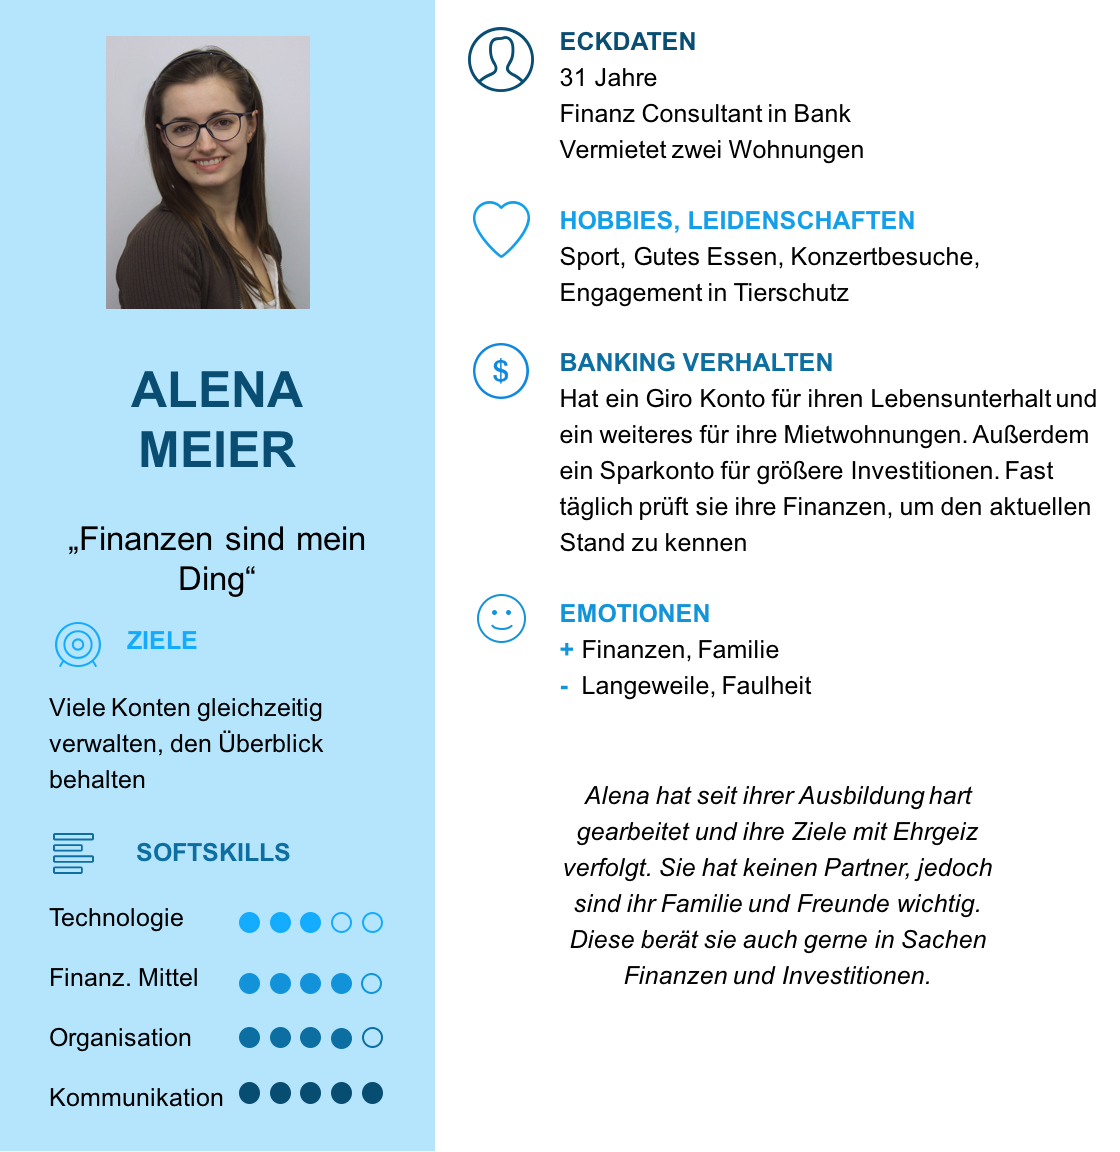
\includegraphics[width=1.0\textwidth]{bilder/3_alenaMeier.png}}
    \caption{Persona Alena Meier}
    \label{fig:alena-meier-anhang}
\end{figure}

\begin{figure}[!htb]
    \centering
    \fbox{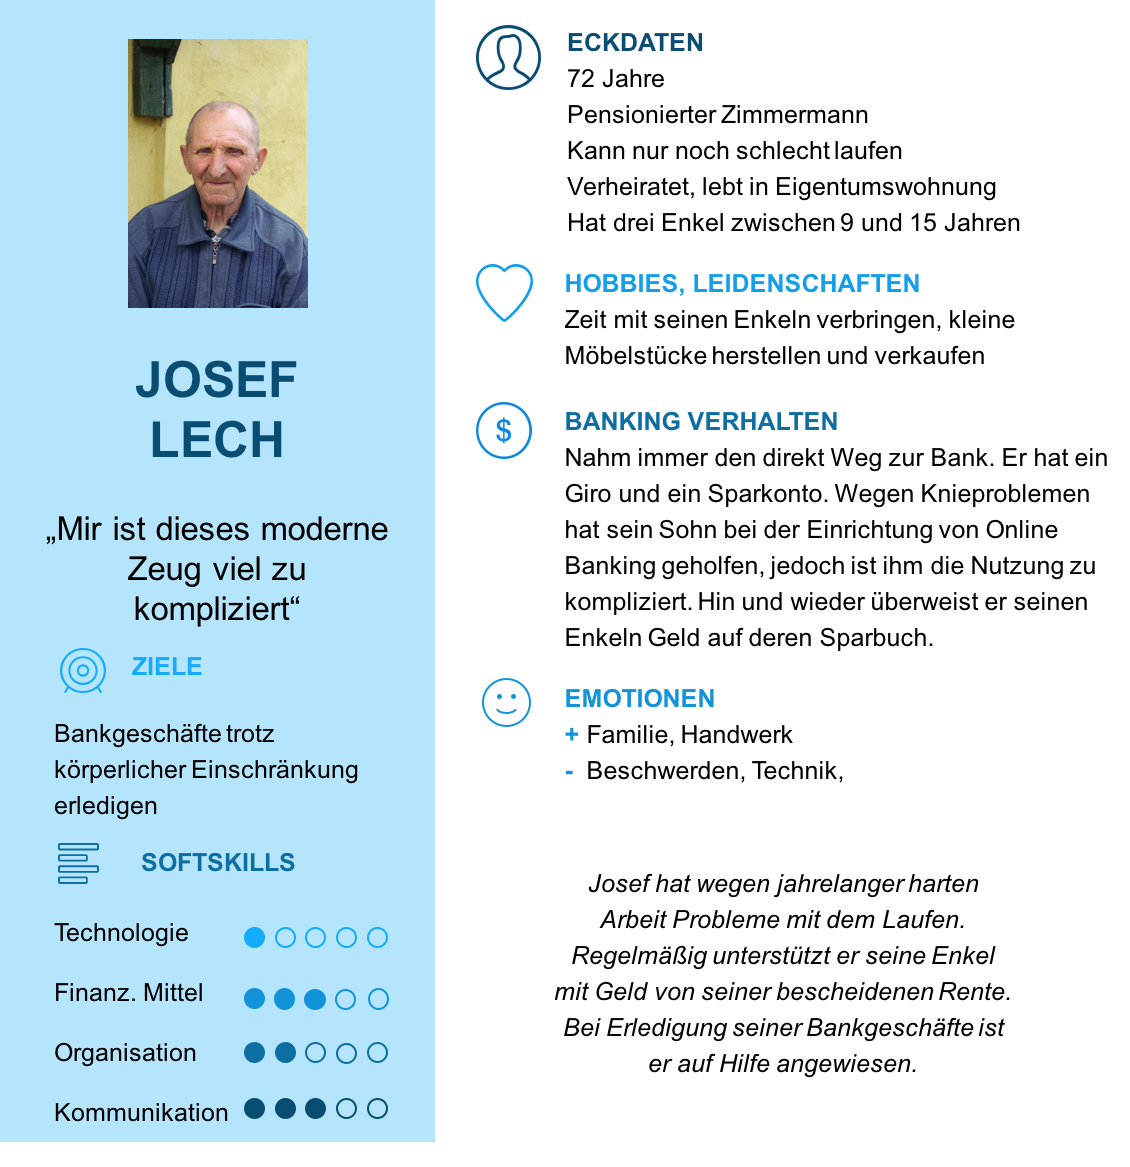
\includegraphics[width=1.0\textwidth]{bilder/3_josefLech.png}}
    \caption{Persona Josef Lech}
    \label{fig:josef-lech}
\end{figure}

\begin{figure}[!htb]
    \centering
    \fbox{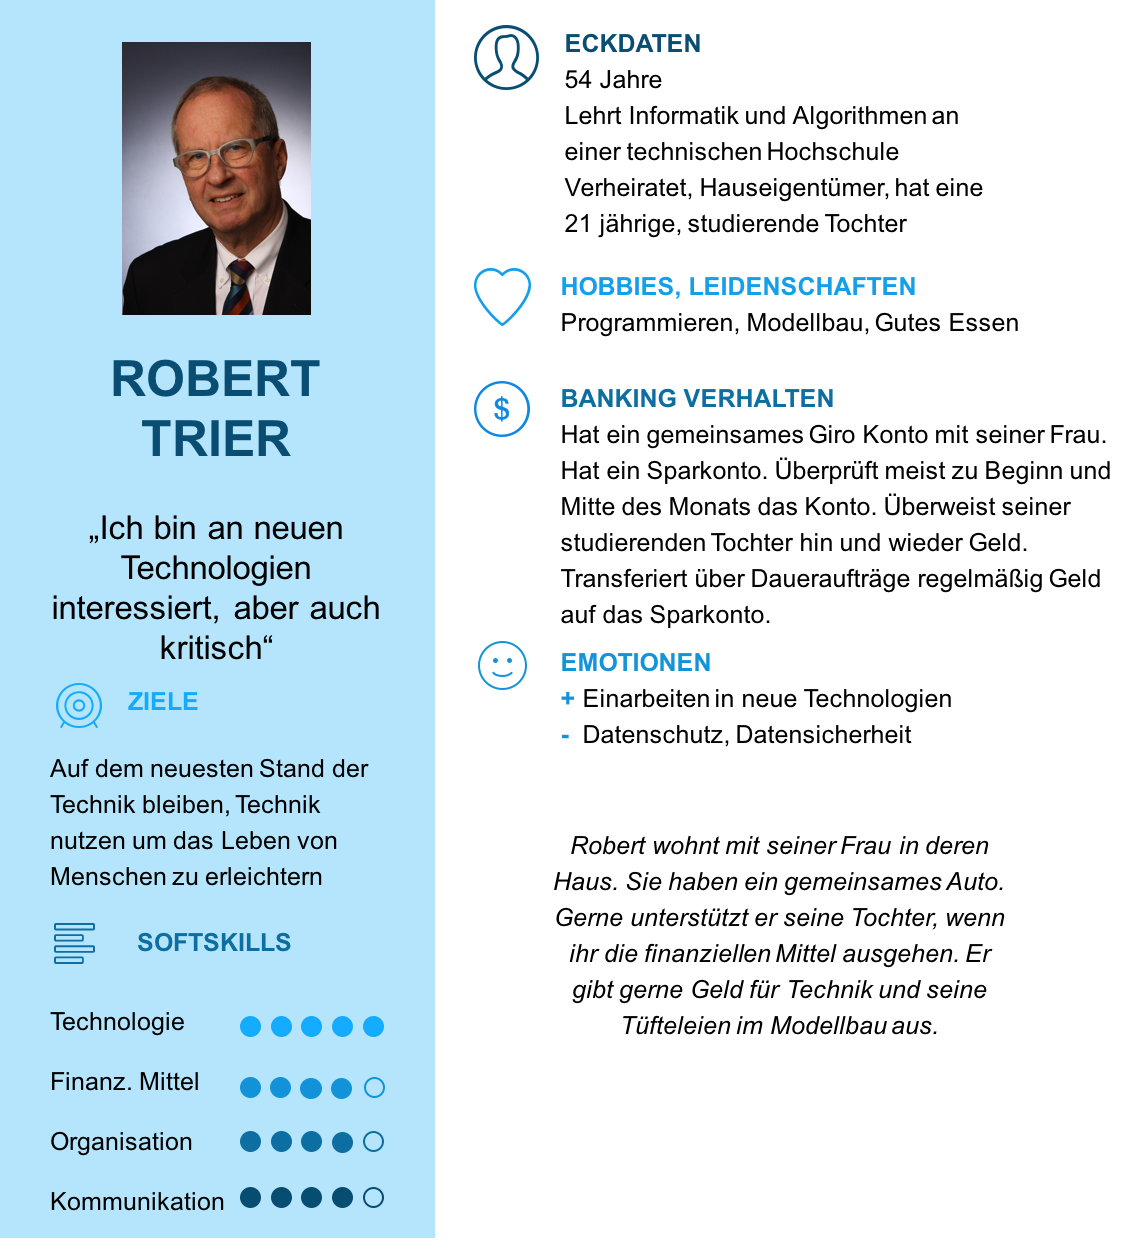
\includegraphics[width=1.0\textwidth]{bilder/3_robertTrier.png}}
    \caption{Persona Robert Trier}
    \label{fig:robert-trier}
\end{figure}

\begin{figure}[!htb]
    \centering
    \fbox{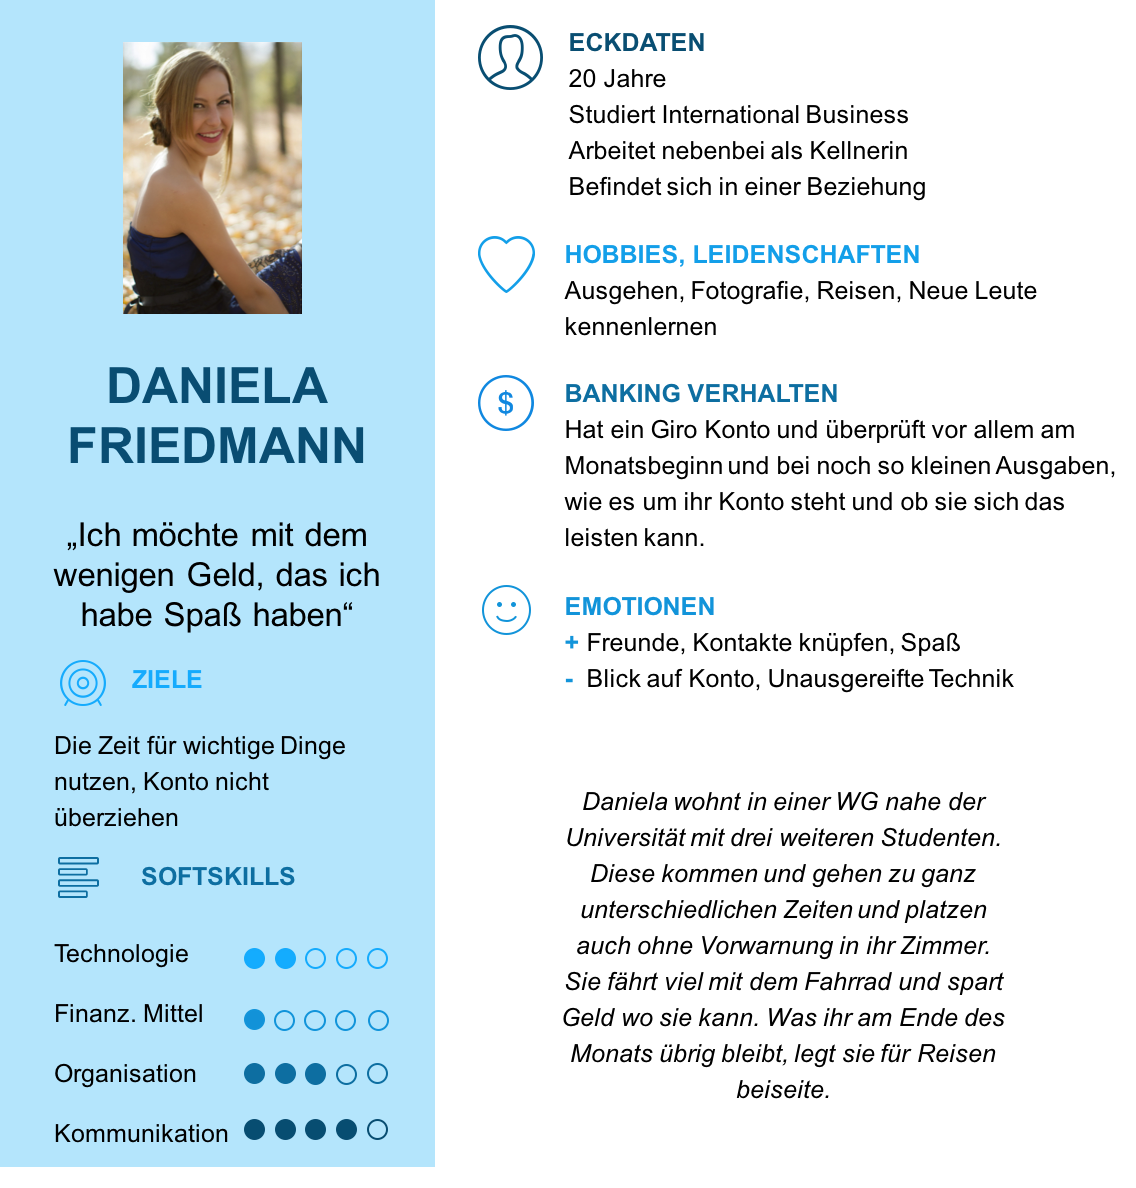
\includegraphics[width=1.0\textwidth]{bilder/3_danielaFriedmann.png}}
    \caption{Persona Daniela Friedmann}
    \label{fig:daniela-friedmann}
\end{figure}

\section{Liste der User Stories}
\label{sec:anhang-user-stories}
Im Folgenden sind alle identifizierten User Stories und etwaige Akzeptanzkriterien aufgeführt. Aus Platz- und Übersichtlichkeitsgründen stellen diese nur den aktuellen Stand dar. Die initiale Version aus Kapitel \ref{subsec:user-stories} und etwaige Zwischenstände sind hier nicht dokumentiert. Änderungen sind mit Referenz auf die Story in den jeweiligen Kapiteln genauer beschrieben.

\begin{enumerate}
\item\textbf{Hilfe aufrufen}: Als allgemeiner Benutzer, möchte ich mir Hilfestellung ausgeben lassen, um in Erfahrung zu bringen, welche Funktionen der Anwendung ich mit welchen Formulierungen verwenden kann.

\item\textbf{Profil anlegen}: Als allgemeiner Benutzer, möchte ich ein Profil anlegen, um für die Nutzung der Anwendung zu registrieren.

\item\textbf{Profil bearbeiten}: Als authentifizierter Benutzer, möchte ich mein Profil bearbeiten, um Änderungen daran vorzunehmen.

\item\textbf{Profil löschen}: Als authentifizierter Benutzer, möchte ich mein Profil löschen, um die Nutzung der Anwendung über dieses Profil einzustellen.

\item\textbf{Authentifizierung durchführen}: Als registrierter Benutzer, möchte ich mich authentifizieren, um den vollen Funktionsumfang der Anwendung nutzen zu können.

\item\textbf{Bankkonto anbinden}: Als authentifizierter Benutzer, möchte ich beliebige Bankkonten mit dem System verknüpfen, um diese mit der Anwendung verwalten zu können.

\item\textbf{Bankkonto-Verknüpfung bearbeiten}: Als authentifizierter Benutzer, möchte ich Bankkonten-Verknüpfungen bearbeiten, um den Namen der Konten zu ändern.

\item\textbf{Bankkonto-Verknüpfung löschen}: Als authentifizierter Benutzer, möchte ich Bankkonten-Verknüpfungen löschen, um die Anbindung für dieses Konto aufzuheben.

\item\textbf{Hauptkonto wählen}: Als authentifizierter Benutzer, möchte ich eines meiner Konten als Hauptkonto setzen, um Transaktionen und Berechnungen automatisch von diesem Konto aus ausführen zu lassen.

\item\textbf{Vorlagen anlegen}: Als authentifizierter Benutzer, möchte ich beliebig viele Überweisungs-Vorlagen anlegen, um Transaktionen durchführen zu können.

\item\textbf{Vorlagen bearbeiten}: Als authentifizierter Benutzer, möchte ich Überweisungs-Vorlagen bearbeiten, um Änderungen daran vorzunehmen.

\item\textbf{Vorlagen löschen}: Als authentifizierter Benutzer, möchte ich Überweisungs-Vorlagen löschen, um die Verwendung nicht genutzter Vorlagen einzustellen.

\item\textbf{Kontostand abfragen}: Als authentifizierter Benutzer, möchte ich den Kontostand abfragen, um herauszufinden wie viel Geld ich aktuell auf dem Konto habe.

\item\textbf{Transaktion via Vorlage tätigen}: Als authentifizierter Benutzer, möchte ich mit Hilfe der Überweisungsvorlagen Transaktionen durchführen, um schnell Geld an den in der Vorlage definierten Kontoinhaber zu überweisen.

\item\textbf{Transaktion via IBAN tätigen}: Als authentifizierter Benutzer, möchte ich mit Hilfe einer IBAN Transaktionen durchführen, um Geld an den Kontoinhaber dieser IBAN zu überweisen.

\item\textbf{TAN eingeben}: als authentifizierter Benutzer, möchte ich die die TAN Nummer für eine getätigte Transaktion eingeben, um diese Transaktion zu bestätigen.

\item\textbf{Gehaltseingang prüfen}: Als authentifizierter Benutzer, möchte ich ich prüfen, ob mein Gehalt überwiesen wurde, um dessen Eingang schnell und ohne Nennung der Höhe des Betrages abzufragen.

\item\textbf{Höhe des Gehaltes prüfen}: Als authentifizierter Benutzer, möchte ich ich abrufen, wie hoch mein Gehalt ist, um zu prüfen, ob es korrekt verrechnet wurde.

\item\textbf{Datum des Gehaltes prüfen}: Als authentifizierter Benutzer, möchte ich ich abrufen, wann mein Gehalt überwiesen wurde, um zu prüfen, ob mein Arbeitgeber rechtzeitig überwiesen hat.

\item\textbf{Budget abrufen}: Als authentifizierter Benutzer, möchte ich wissen wie viel Geld ich bis Ende der aktuellen Finanzperiode zur Verfügung habe, um mein Ausgabeverhalten entsprechend anpassen zu können.

\item\textbf{Budget von letztem Monat abrufen}: Als authentifizierter Benutzer, möchte ich wissen wie viel Geld ich bis Ende des letzten Monates hatte, um zu prüfen, ob Änderungen in meinem Ausgabeverhalten Wirkung zeigen.

\item\textbf{Fixkosten prüfen}: Als authentifizierter Benutzer, möchte ich die Höhe und Art meiner Fixkosten wissen, um in Erfahrung zu bringen wofür ich regelmäßig wieviel Geld ausgebe.

\item\textbf{Umsatzdaten prüfen}: Als authentifizierter Benutzer, möchte ich Informationen zu Umsatzdaten abfragen, um in Erfahrung zu bringen, ob bestimmte Transaktionen durchgeführt wurden.

\item\textbf{Sparziele anlegen}: Als authentifizierter Benutzer, möchte ich auf verknüpften Sparkonten Sparziele anlegen, um für ein von mir festgelegtes Thema Geld zu sparen.

\item\textbf{Sparziele bearbeiten}: Als authentifizierter Benutzer, möchte ich Betrag, Intervall und Name von angelegten Sparzielen bearbeiten, um diese auf meine aktuellen Bedürfnisse anzupassen.

\item\textbf{Sparziele löschen}: Als authentifizierter Benutzer, möchte ich angelegte Sparziele löschen, um die Sparmaßnahmen für dieses Ziel einzustellen.

\item\textbf{Sparziele ausgeben}: Als authentifizierter Benutzer, möchte ich angelegte Sparziele ausgeben lassen, um in Erfahrung zu bringen, wofür ich bisher spare.

\item\textbf{Ausgaben der letzten Finanzperiode}: Als authentifizierter Benutzer möchte ich wissen, wie viel Geld ich in der letzten Finanzperiode insgesamt ausgegeben habe, um mein Ausgabeverhalten im Blick zu haben.
\end{enumerate}

\section{Liste aller Szenarien}
\label{sec:anhang-szenarien}
Im Folgenden werden alle entwickelten Szenarien aus Kapitel \ref{subsec:szenarien} dargestellt. 

\begin{figure}[!htb]
    \centering
    \fbox{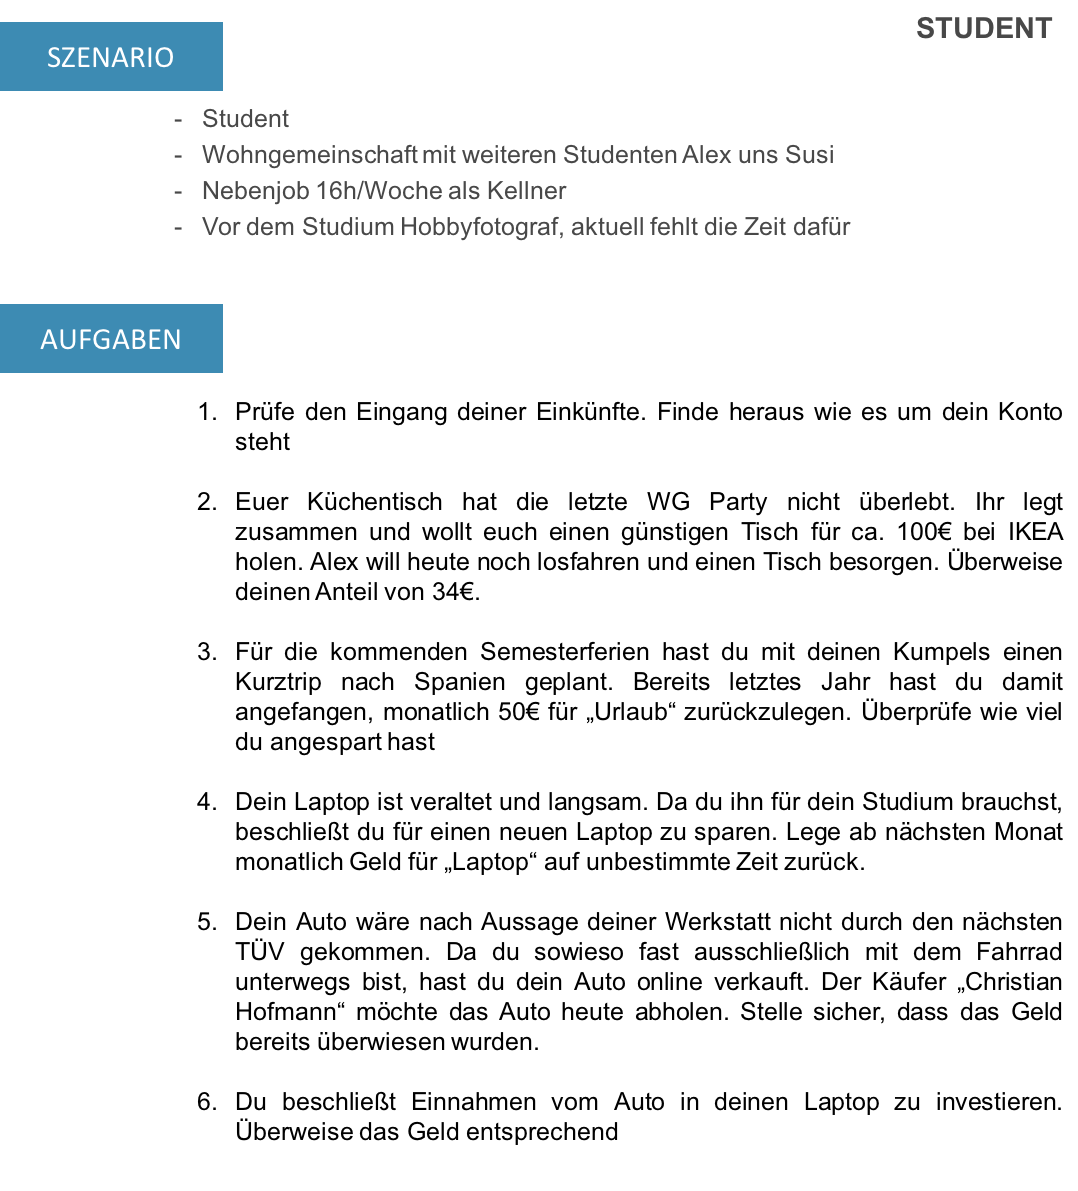
\includegraphics[width=1.0\textwidth]{bilder/3_szenarioStudent.png}}
    \caption{Studenten Szenario}
    \label{fig:szenario-student}
\end{figure}

\begin{figure}[!htb]
    \centering
    \fbox{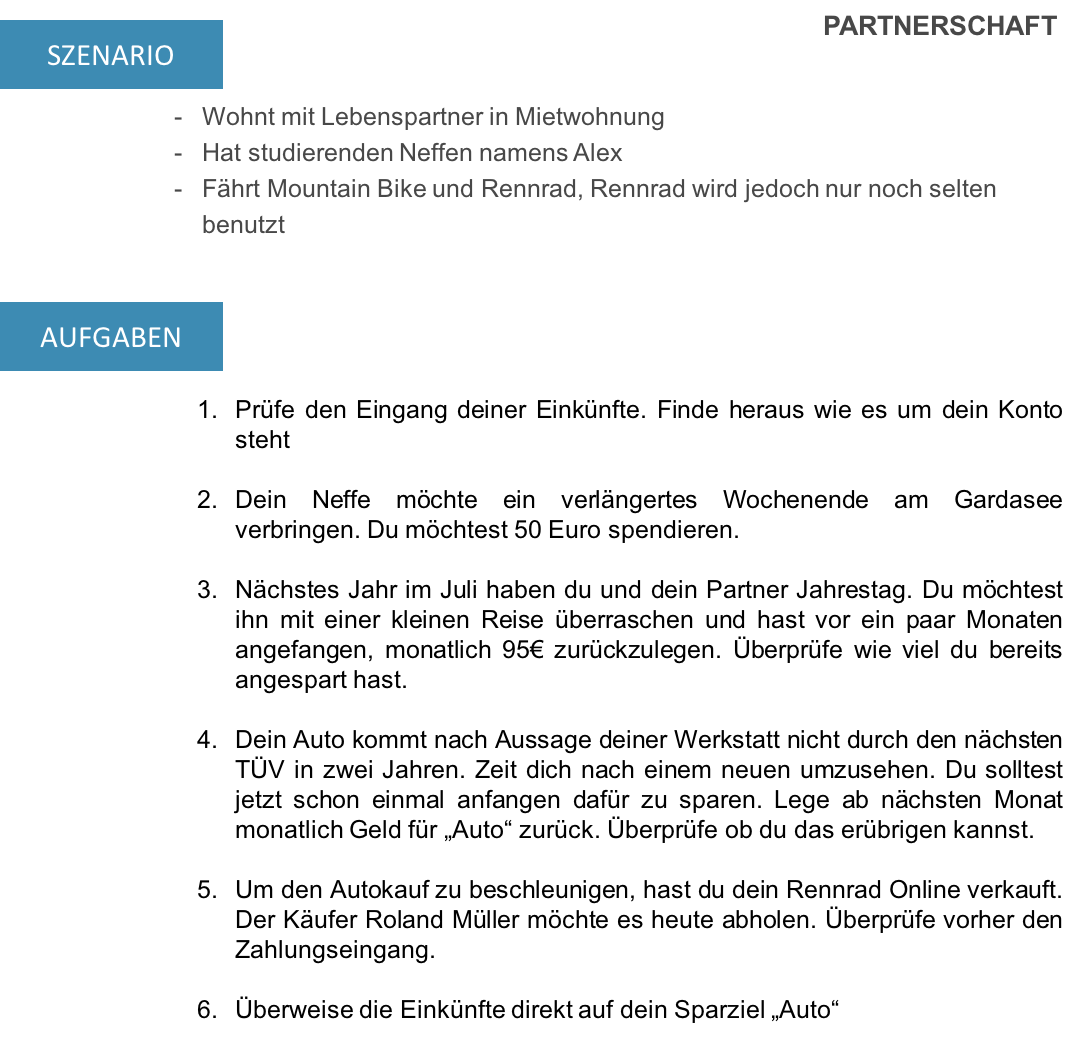
\includegraphics[width=1.0\textwidth]{bilder/3_szenarioPartner.png}}
    \caption{Partnerschaft Szenario}
    \label{fig:szenario-partner-anhang}
\end{figure}

\begin{figure}[!htb]
    \centering
    \fbox{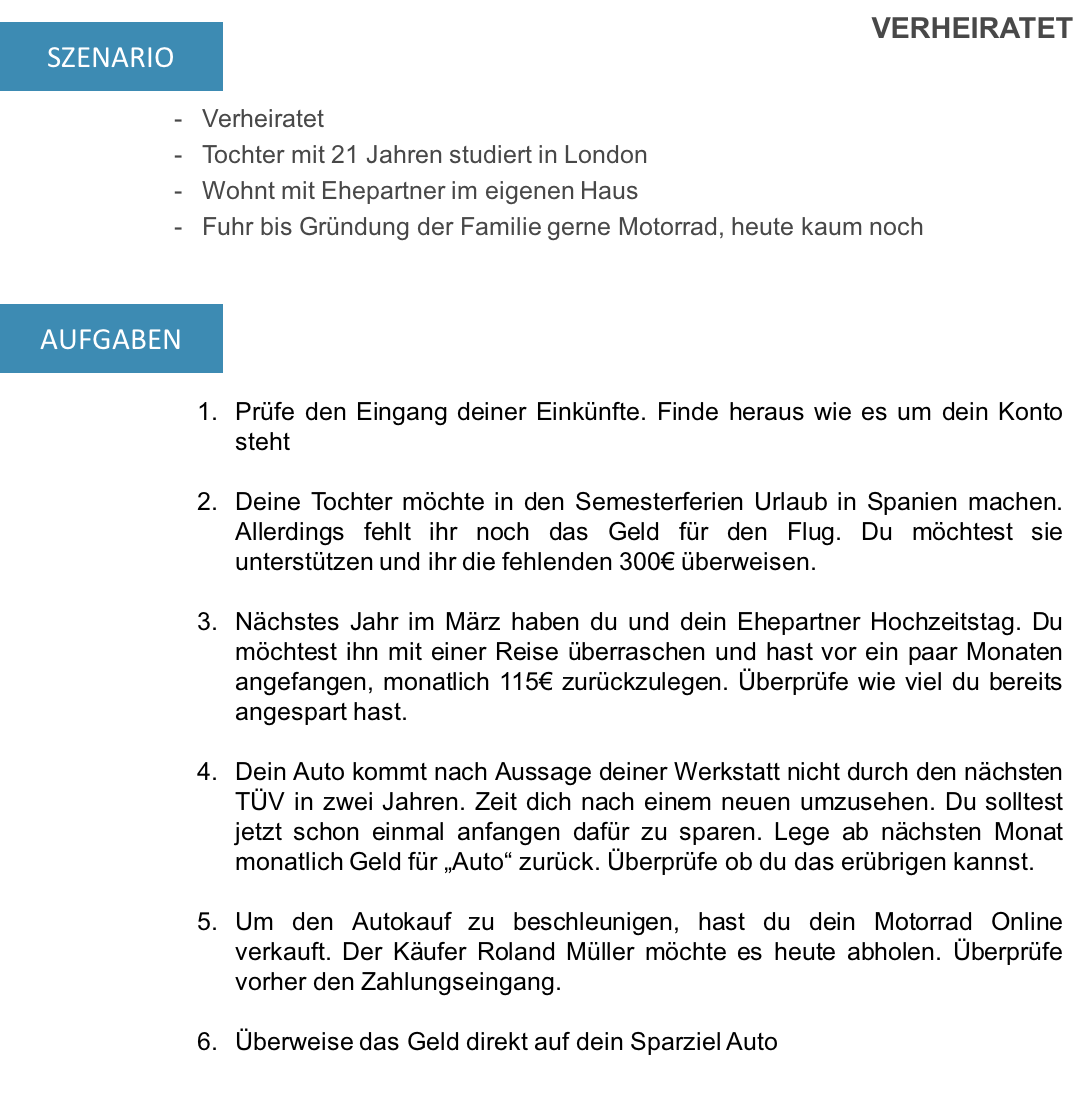
\includegraphics[width=1.0\textwidth]{bilder/3_szenarioVerheiratet.png}}
    \caption{Verheiratet Szenario}
    \label{fig:szenario-verheiratet}
\end{figure}

\section{Communication Prototyping Tool Skript Schema}
\label{sec:cpt-input-schema}

Im Folgenden ist das Schema des Skriptes defniert, das vom CPT Tool für den Aufbau der Oberfläche verwendet wird.

\lstinputlisting[caption={Skript Schema der cft Ausgabe}]{docs/conversationPrototypingDocument.cft.json}

\section{Konzept}
\label{sec:anhang-konzept}
Die folgenden Abbildungen zeigen die ausgearbeiteten Intents und bilden das Bedienkonzept. Sie sind das Ergebnis der empirischen Daten und User Tests. Diese bilden die Basis für die Implementierung in Kapitel \ref{cha:umsetzung}.

\begin{figure}[!htb]
    \centering
    \fbox{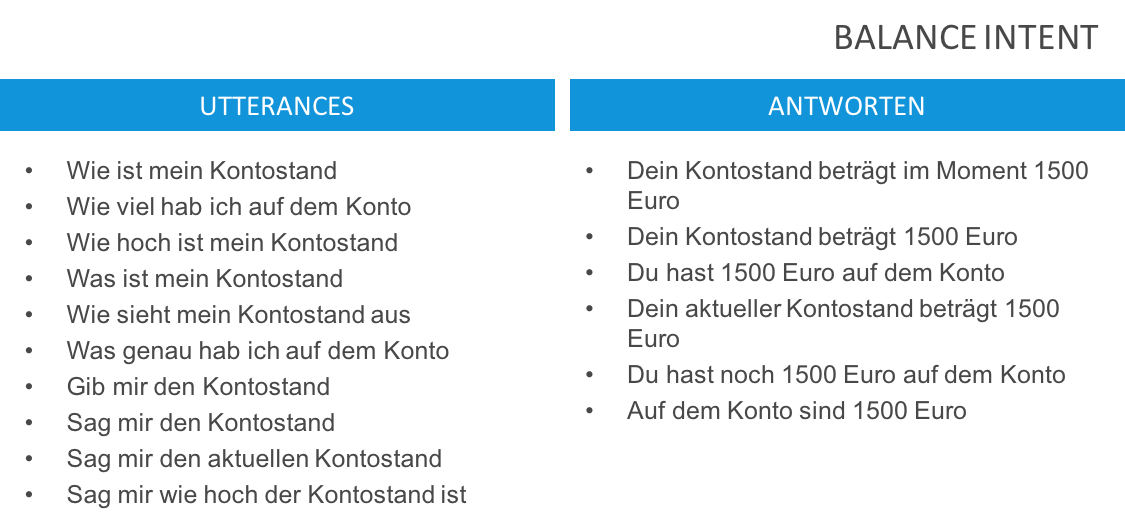
\includegraphics[width=1.0\textwidth]{bilder/3_conceptBalance.png}}
    \caption{Kontostand Intent}
    \label{fig:concept-balance}
\end{figure}

\begin{figure}[!htb]
    \centering
    \fbox{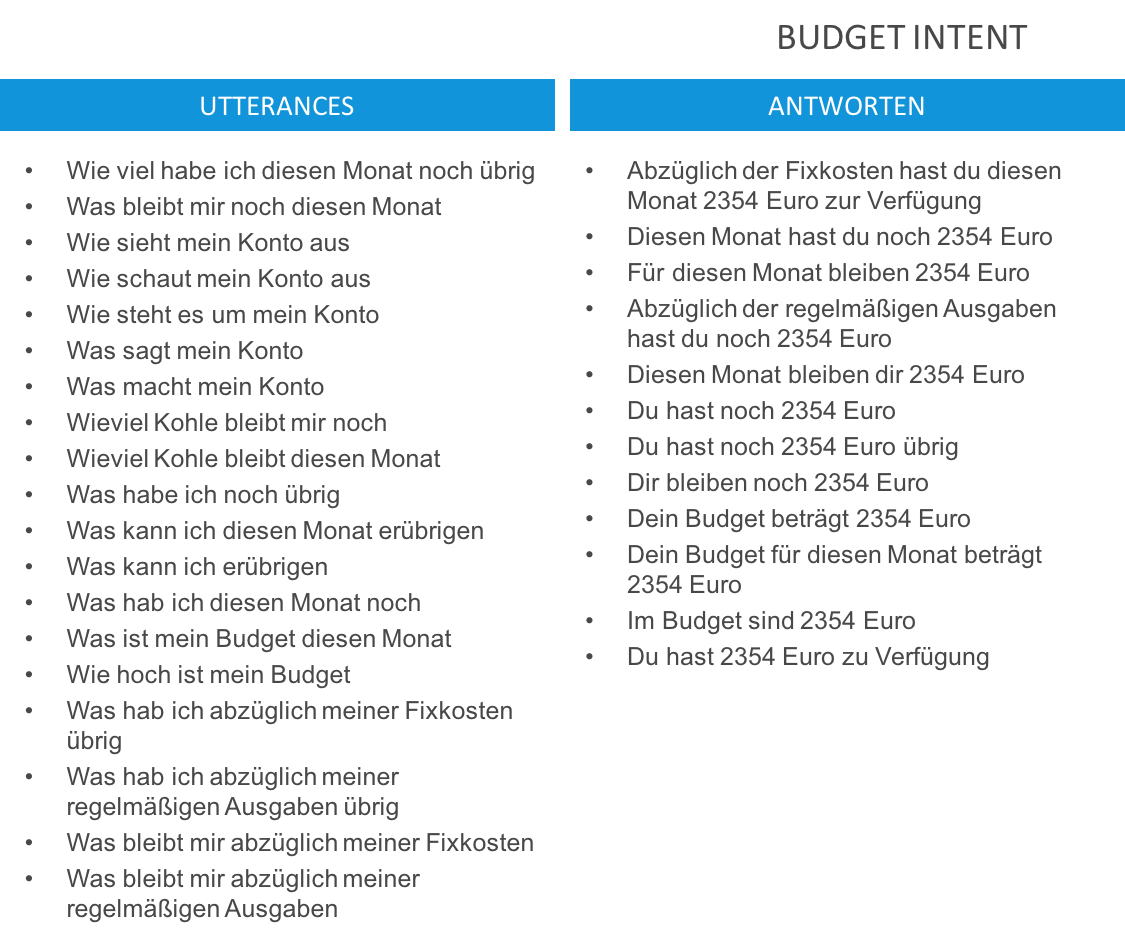
\includegraphics[width=1.0\textwidth]{bilder/3_conceptBudget.png}}
    \caption{Budget Intent}
    \label{fig:concept-budget}
\end{figure}

\begin{figure}[!htb]
    \centering
    \fbox{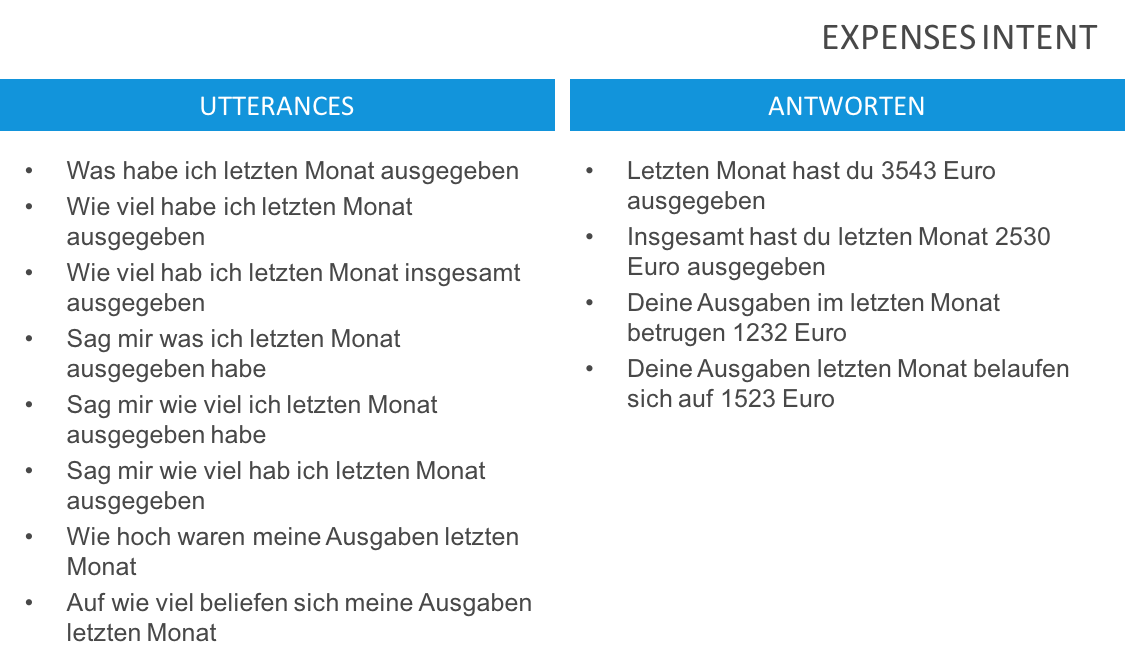
\includegraphics[width=1.0\textwidth]{bilder/3_conceptExpenses.png}}
    \caption{Ausgaben Intent}
    \label{fig:concept-expenses}
\end{figure}

\begin{figure}[!htb]
    \centering
    \fbox{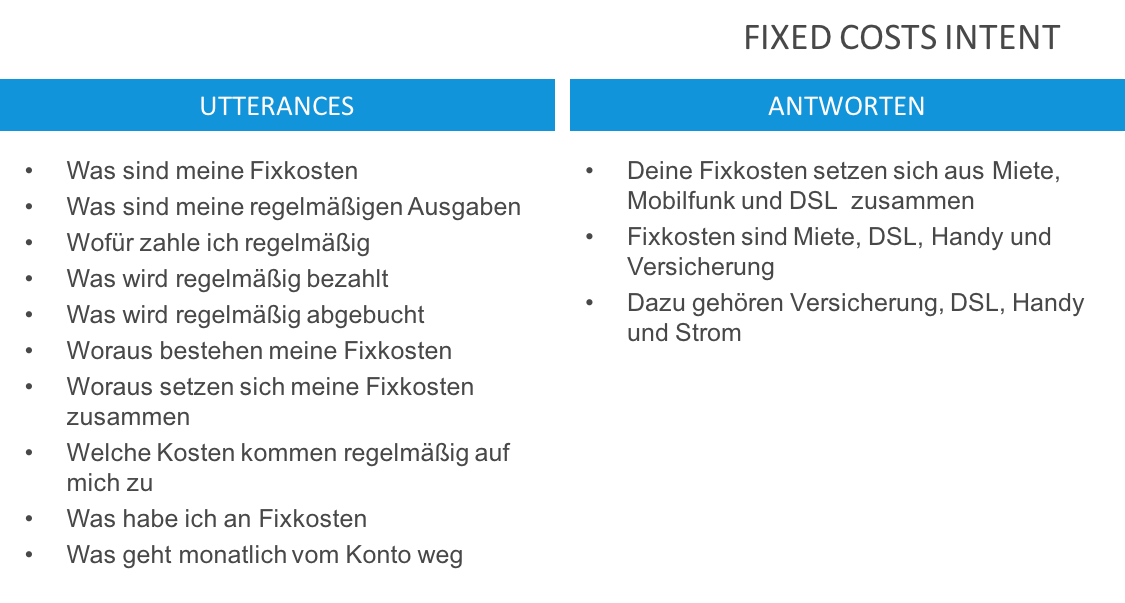
\includegraphics[width=1.0\textwidth]{bilder/3_conceptFixedCosts.png}}
    \caption{Fixkosten Intent}
    \label{fig:concept-fixedcosts}
\end{figure}

\begin{figure}[!htb]
    \centering
    \fbox{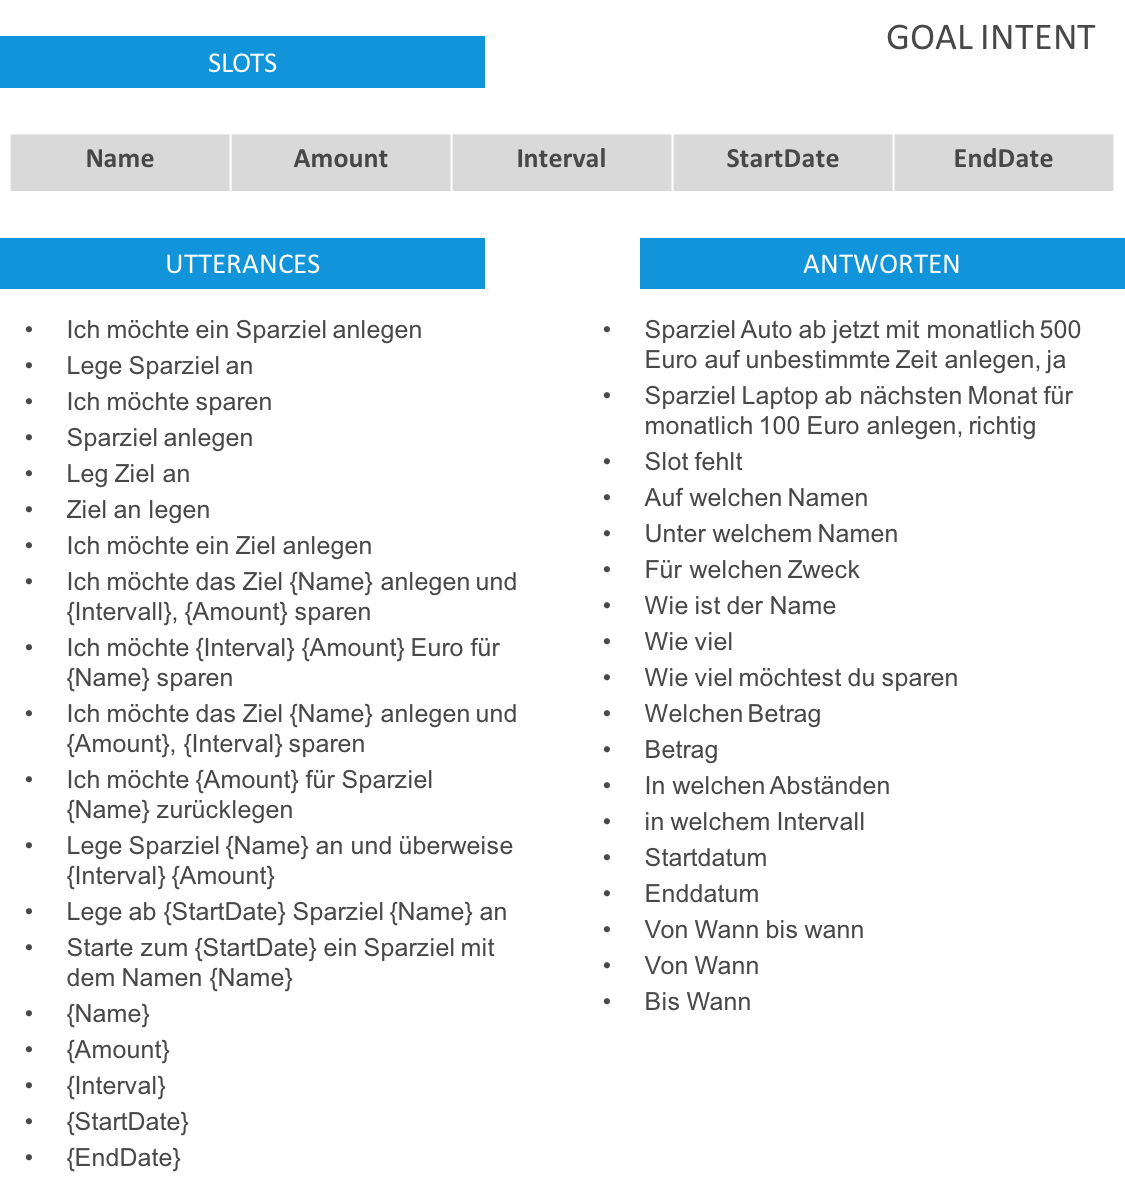
\includegraphics[width=1.0\textwidth]{bilder/3_conceptGoal.png}}
    \caption{Sparziel Intent}
    \label{fig:concept-goal}
\end{figure}

\begin{figure}[!htb]
    \centering
    \fbox{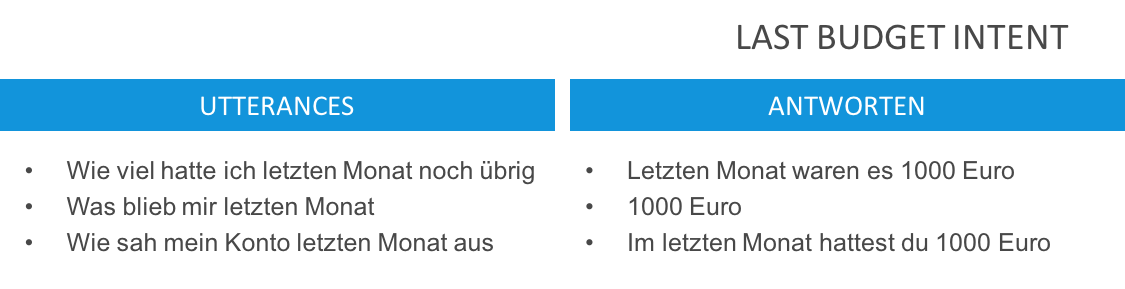
\includegraphics[width=1.0\textwidth]{bilder/3_conceptLastBudget.png}}
    \caption{Letztes Budget Intent}
    \label{fig:concept-lastbudget}
\end{figure}

\begin{figure}[!htb]
    \centering
    \fbox{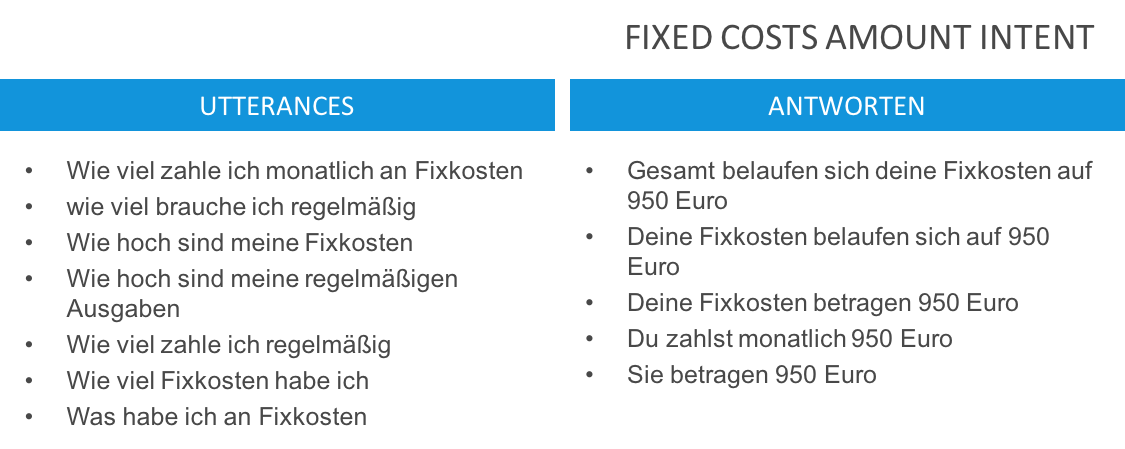
\includegraphics[width=1.0\textwidth]{bilder/3_conceptFixedCostsAmount.png}}
    \caption{Fixkosten Betrag Intent}
    \label{fig:concept-fixedcosts-amount}
\end{figure}

\begin{figure}[!htb]
    \centering
    \fbox{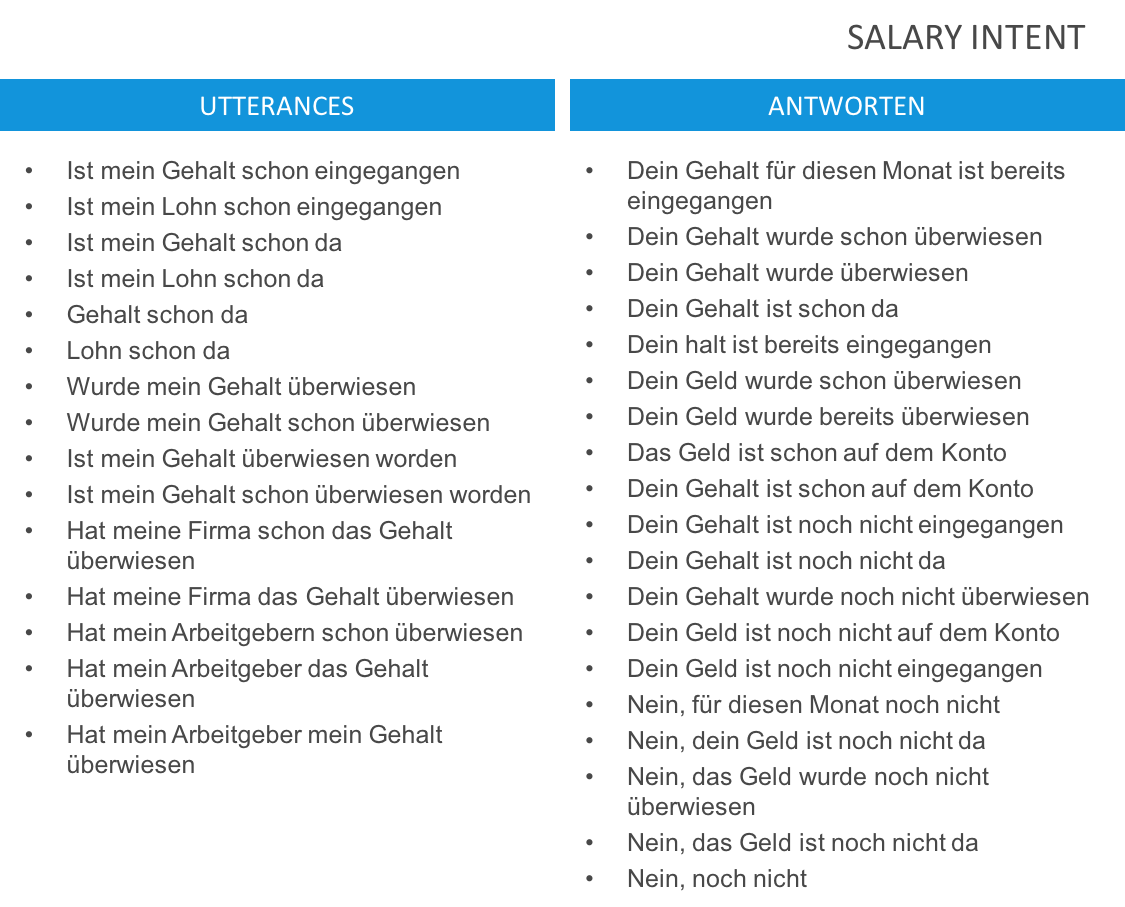
\includegraphics[width=1.0\textwidth]{bilder/3_conceptSalary.png}}
    \caption{Gehaltseingang Intent}
    \label{fig:concept-salary}
\end{figure}

\begin{figure}[!htb]
    \centering
    \fbox{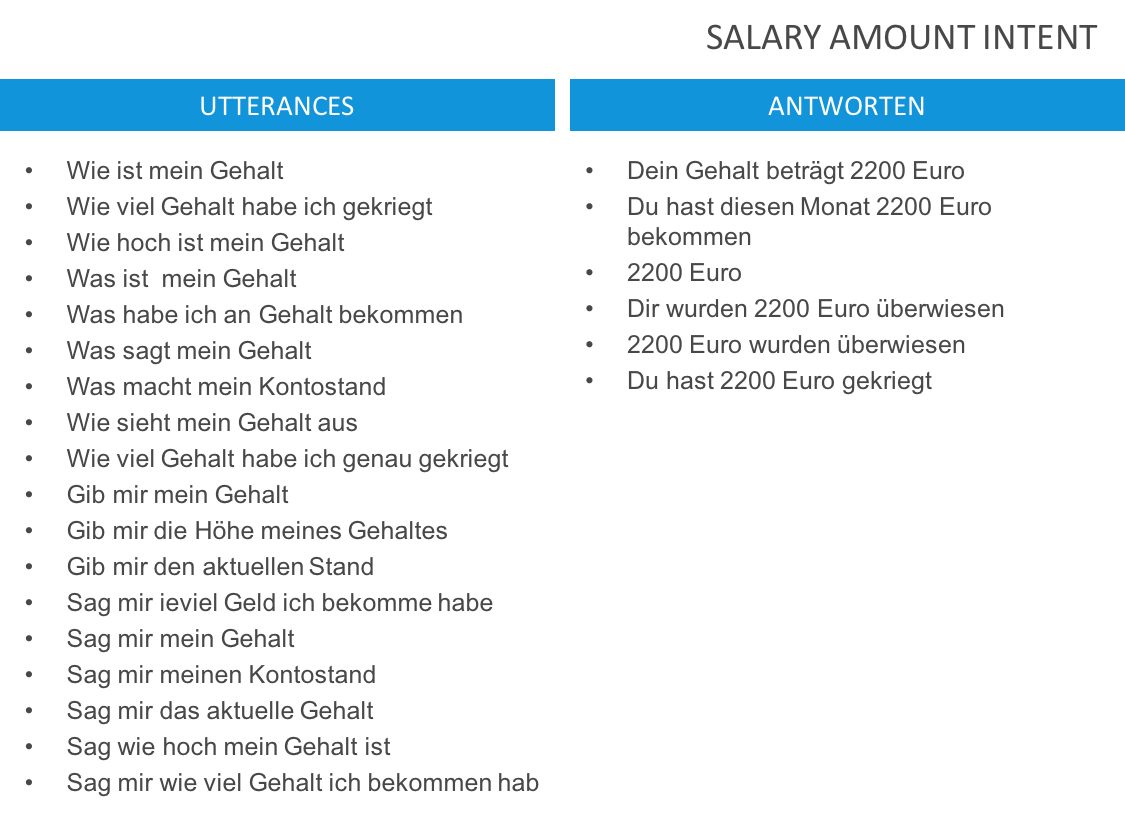
\includegraphics[width=1.0\textwidth]{bilder/3_conceptSalaryAmount.png}}
    \caption{Gehalt Betrag Intent}
    \label{fig:concept-salary-amount}
\end{figure}

\begin{figure}[!htb]
    \centering
    \fbox{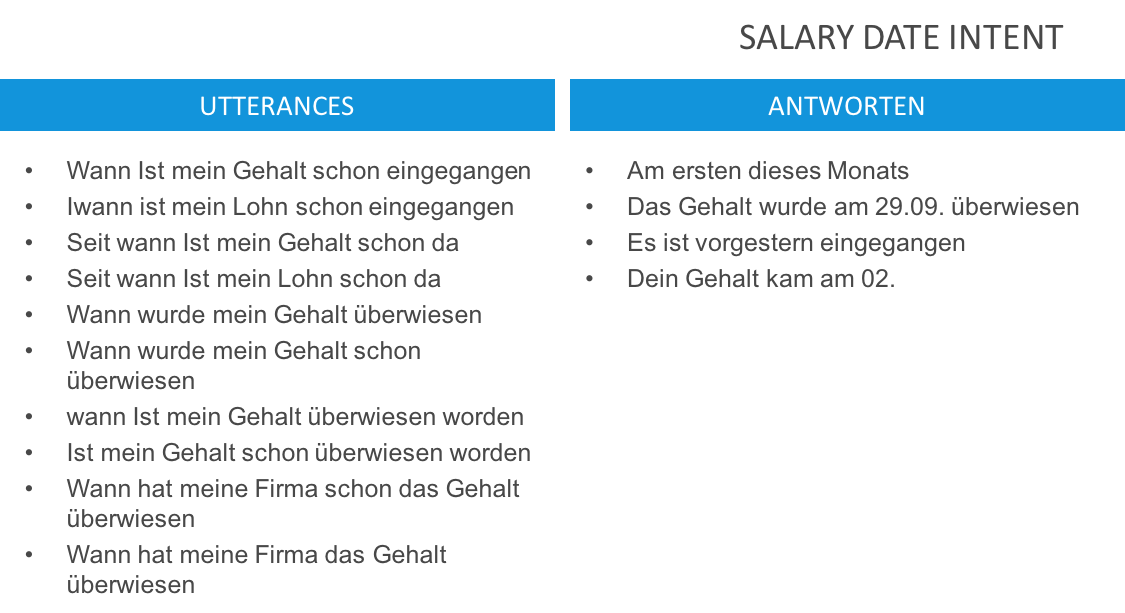
\includegraphics[width=1.0\textwidth]{bilder/3_conceptSalaryDate.png}}
    \caption{Gehalt Datum Intent}
    \label{fig:concept-salary-date}
\end{figure}

\begin{figure}[!htb]
    \centering
    \fbox{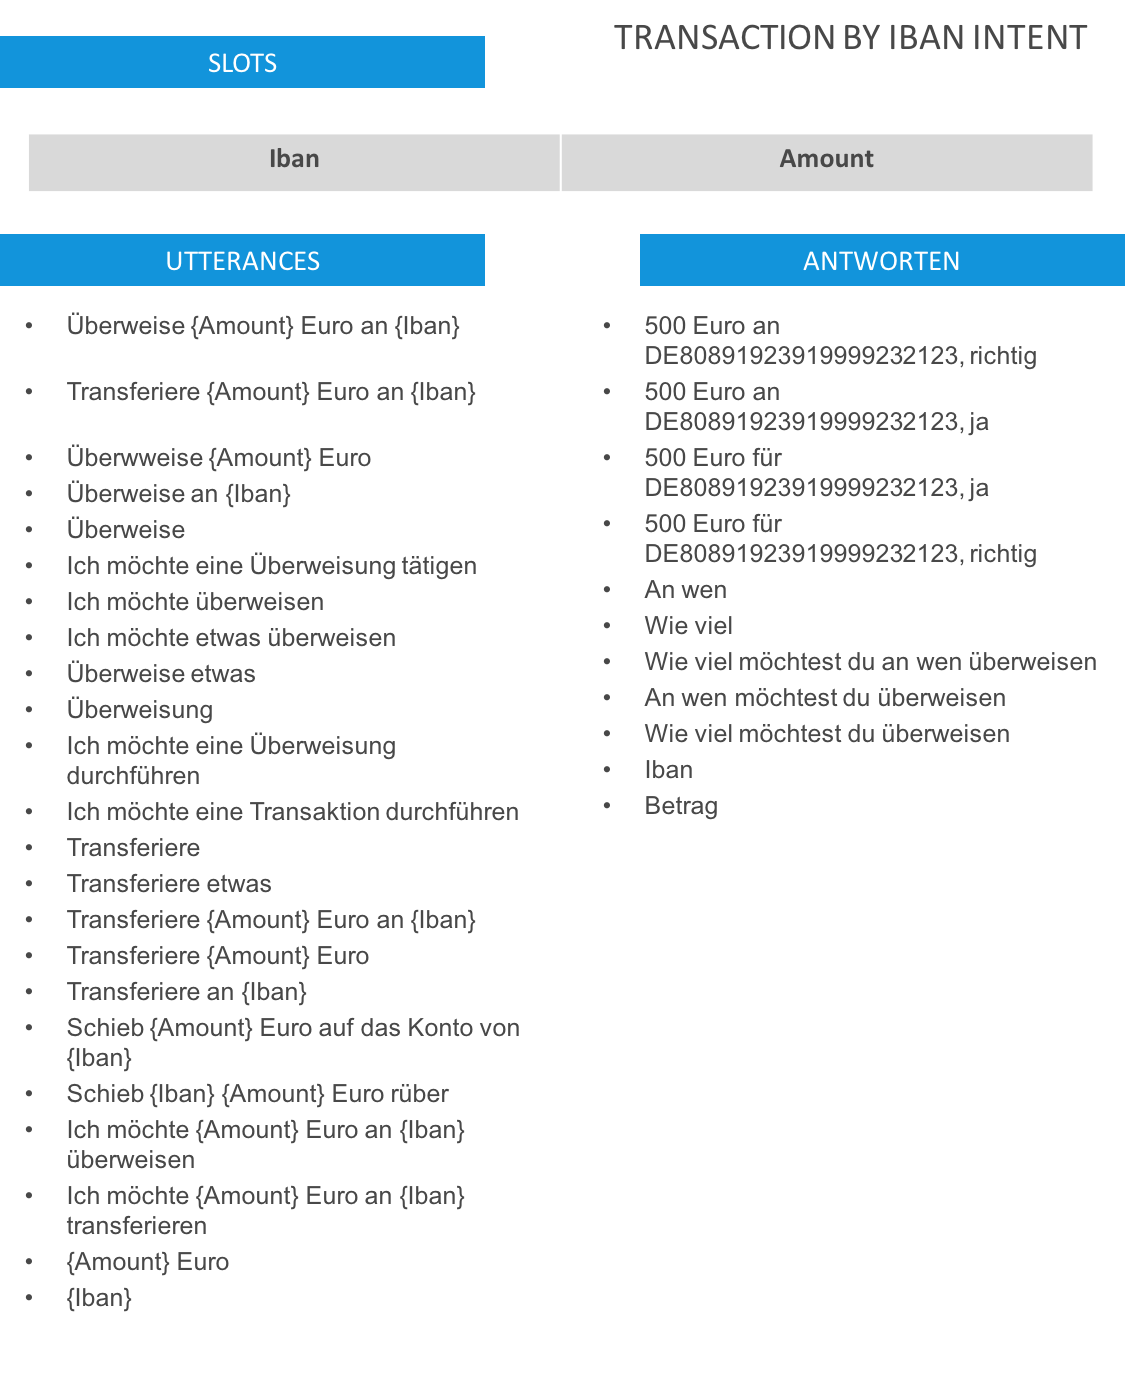
\includegraphics[width=1.0\textwidth]{bilder/3_conceptTransactionIban.png}}
    \caption{Transaktion via Iban Intent}
    \label{fig:concept-transaction-iban}
\end{figure}

\begin{figure}[!htb]
    \centering
    \fbox{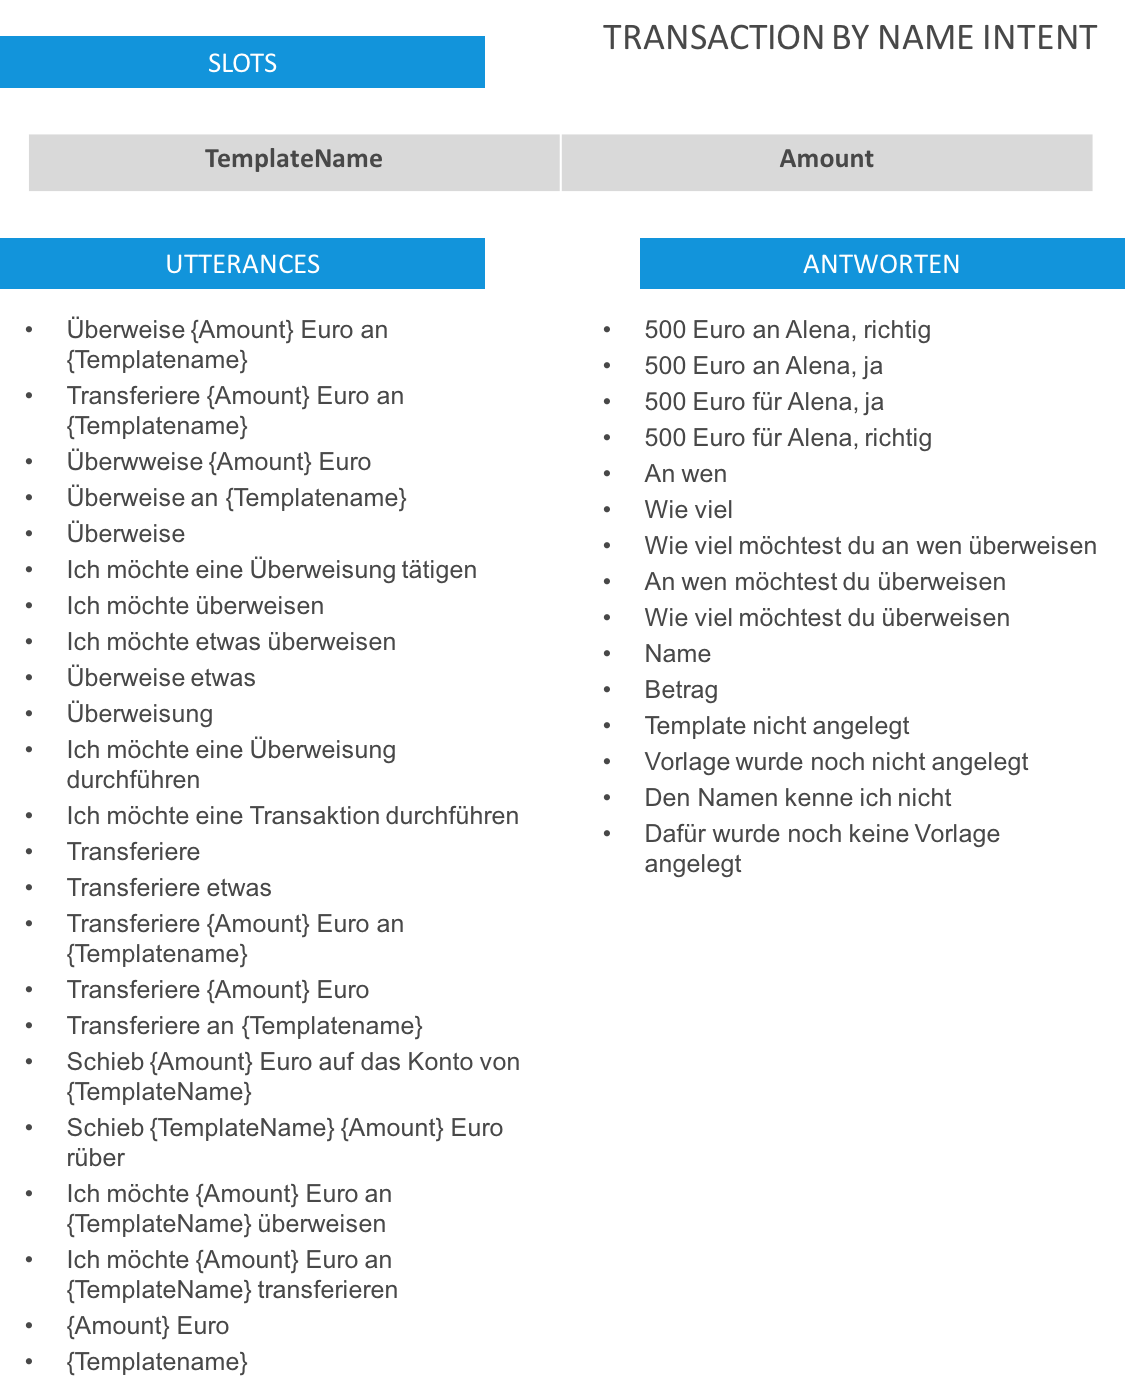
\includegraphics[width=1.0\textwidth]{bilder/3_conceptTransactionName.png}}
    \caption{Transaktion Name Intent}
    \label{fig:concept-transaction-name}
\end{figure}

\begin{figure}[!htb]
    \centering
    \fbox{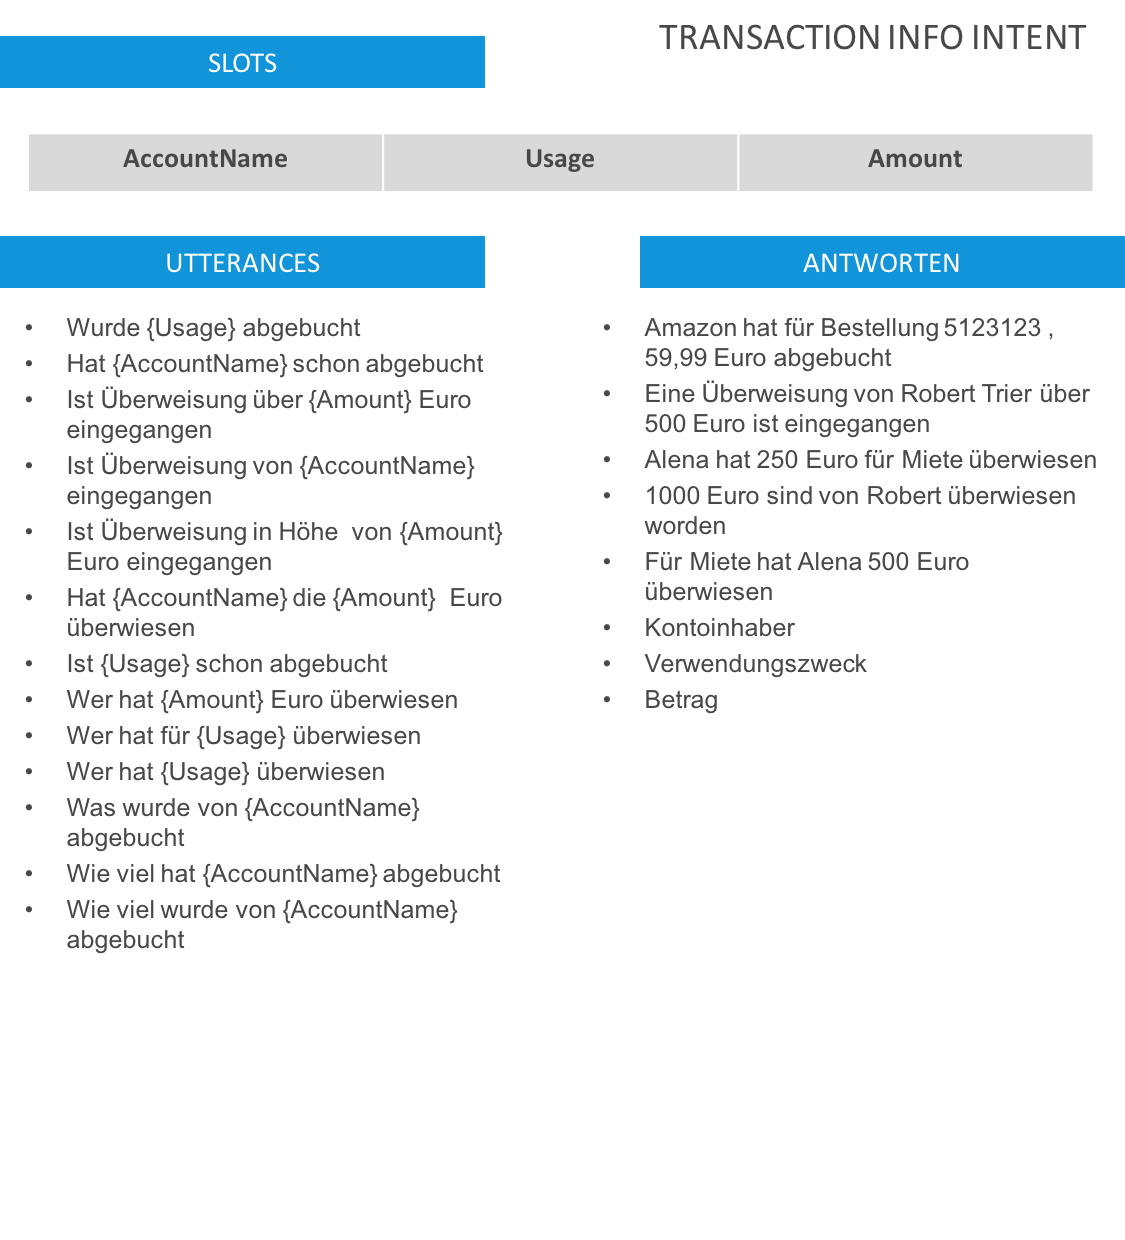
\includegraphics[width=1.0\textwidth]{bilder/3_conceptTransactionInfo.png}}
    \caption{Transaktion Info Intent}
    \label{fig:concept-transaction-info}
\end{figure}

\section{CD Verzeichnisstruktur}
\label{sec:cd-verzeichnisstruktur}
\begin{tabbing}
	mm \= mm \= mmmmmmmmmmmmmmmm \= \kill
    $\vdash$ \textbf{Latex-Files/} $\Rightarrow$ \textit{editierbare \LaTeX~Dateien}\\ %\llcorner
	\> \>  $\vdash$  \textbf{bilder/}   	\> $\Rightarrow$ \textit{Alle verwendeten Bilder}\\
	\> \>  $\vdash$  \textbf{docs/}   	\> $\Rightarrow$ \textit{Sonstige Dokumente}\\
	\> \>  $\vdash$  \textbf{hauptkapitel/}  \> $\Rightarrow$ \textit{Sechs Hauptkapitel}\\
	\> \>  $\vdash$  \textbf{literatur/}   \> $\Rightarrow$ \textit{Bibliotheksdatei und Zitierstil}\\
	\> \>  $\vdash$  \textbf{nebenkapitel/}   \> $\Rightarrow$ \textit{Abstract, Glossar, Erklärung, ...}\\
	\> \> --chronology.sty\\
	\> \> --config.tex\\
	\> \> --main.tex\\
	|\\
	$\vdash$ \textbf{Literatur/} \\ 
	\> \>  $\vdash$  \textbf{Papers/} \\
	\> \>  $\vdash$  \textbf{Websites/} \\ 
	|\\
	$\vdash$ \textbf{Poster/} \\
	\> \>  --Poster.pptx\\
	\> \>  --Poster.pdf\\
	|\\
	$\vdash$ \textbf{Quelltexte/} $\Rightarrow$\\ %\llcorner
	\> \>  $\vdash$  \textbf{cpt/}   	\> $\Rightarrow$ \textit{cpt Anwendung der Prototyping Toolchain}\\
	\> \>  $\vdash$  \textbf{finlexa\_android/}   	\> $\Rightarrow$ \textit{Voice Bank App}\\
	\> \>  $\vdash$  \textbf{finlexa\_central/}   	\> $\Rightarrow$ \textit{Voice Bank Backend}\\
	\> \>  $\vdash$  \textbf{finlexa\_model/}   	\> $\Rightarrow$ \textit{Voice Bank Interaction Model}\\
	\> \>  $\vdash$  \textbf{finlexa\_skill/}  \> $\Rightarrow$ \textit{Voice Bank Skill Server}\\
	\> \>  $\vdash$  \textbf{prototyping\_skripten/}  \> $\Rightarrow$ \textit{Dialogskripten für das Prototyping Tool}\\
	\> \>  $\vdash$  \textbf{prt/}   	\> $\Rightarrow$ \textit{prt Anwendung der Prototyping Toolchain}\\
    |\\
\end{tabbing}
